% !TeX spellcheck = en_US
\documentclass[sigconf,nonacm]{acmart}
\usepackage{listings}
\usepackage{subcaption}
\settopmatter{printacmref=false}
\pagestyle{empty}
\AtBeginDocument{%
  \providecommand\BibTeX{{%
    \normalfont B\kern-0.5em{\scshape i\kern-0.25em b}\kern-0.8em\TeX}}}
\copyrightyear{2020}
\acmYear{2020}
\setcopyright{rightsretained}
\begin{document}
\title{Deep Learning for Visual Computing}
\subtitle{Group 12, Exercise 2: Iterative Optimization and Parametric Models}
\author{SHU Yuting}
\email{e11931687@student.tuwien.ac.at}
\affiliation{Mat.Nr. 11931687}
\author{Helmuth BREITENFELLNER}
\email{helmuth.breitenfellner@student.tuwien.ac.at}
\affiliation{Mat.Nr. 08725866}
\begin{abstract}
In this assignment we have been experimenting with various optimizers,
to better understand their behavior for stochastic gradient
descent.
In addition we were developing deep neural networks, using CNN,
for classifying cats and dogs from images.
Finally, to reduce issues from overfitting, we applied data augmentation,
regularization, early stopping and transfer learning, in various settings.
These experiments were rounded up by looking at the performance of transfer
learning (based on ResNet18) for the classification task.
\end{abstract}
\keywords{Deep Learning, Linear Model, Visual Computing, Image Processing, PyTorch}
\maketitle

\section{Gradient Descent}

Gradient descent is a method for finding the minimum of a function.
It starts at a random position and tries to improve on the position
by going a step into the negative direction of the gradient,
i.e.\ the vector of the partial derivatives of the function.
When the gradient is small enough the assumption is that no further improvement
can be achieved and the current position is returned as the assumed location
of the minimum.

One issue of gradient descent is that it returns potentially any location with zero
gradient as a solution. While at the minimum the gradient is zero, there
are other situations for which this is valid: local mimima, maxima, and saddle points.
Most important for gradient descent are local minima, and most often the solution
returned by gradient descent is a local minimum.

\begin{figure}[h]
  \begin{subfigure}[c]{0.3\columnwidth}
    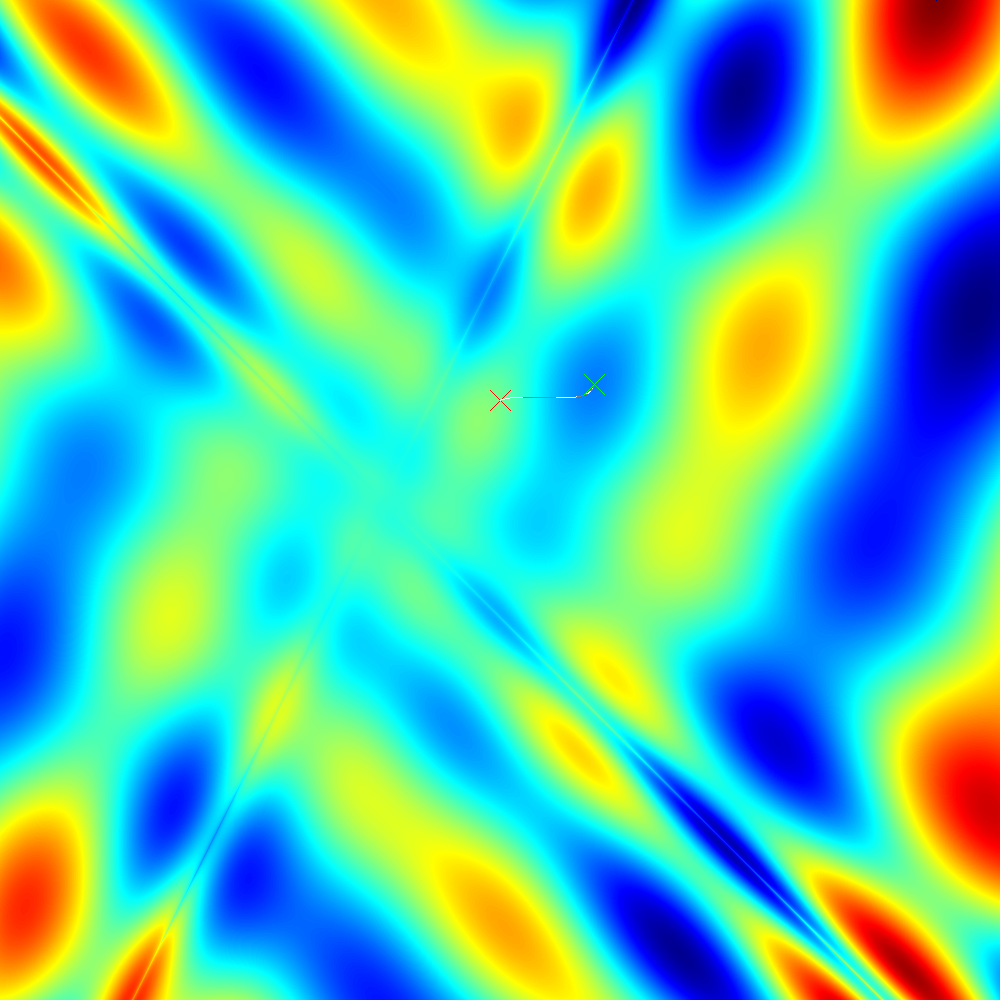
\includegraphics[width=\textwidth]{local-minimum.png}
    \subcaption{Local minima}
  \end{subfigure}
  \hspace{1pt}
  \begin{subfigure}[c]{0.3\columnwidth}
    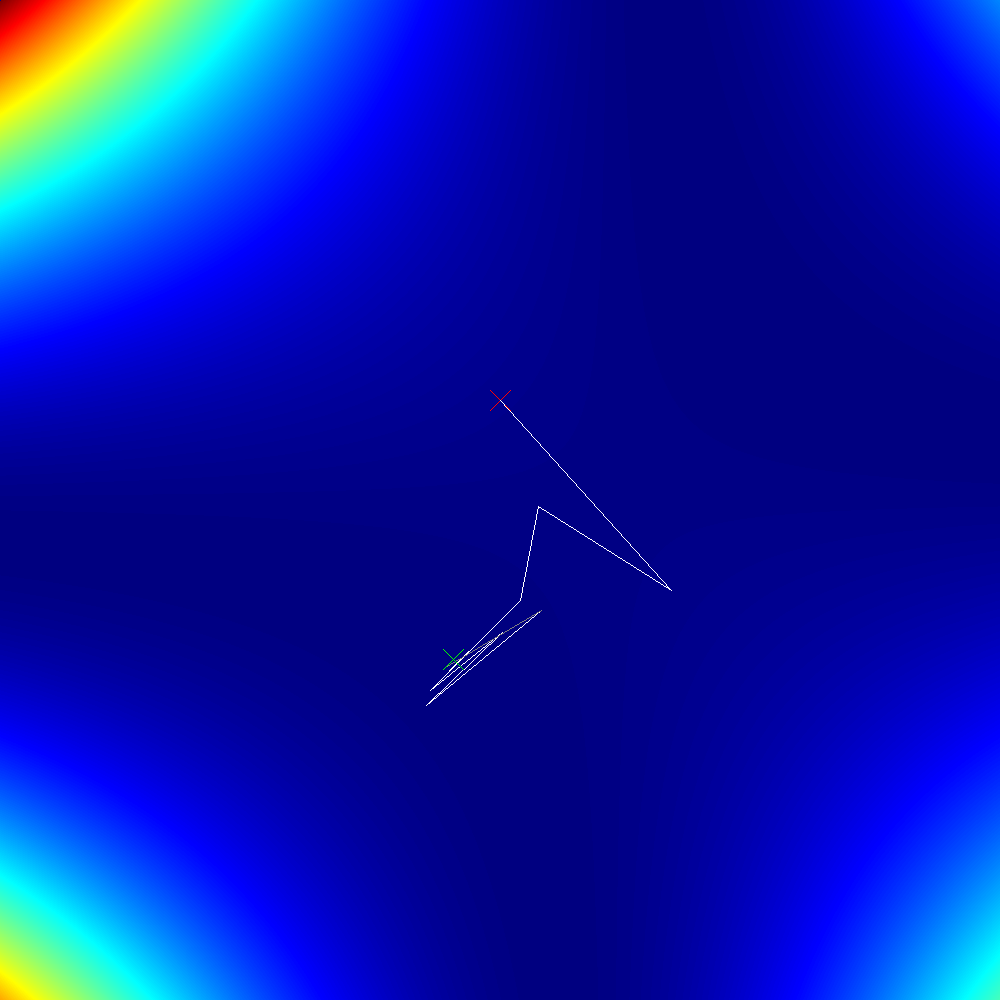
\includegraphics[width=\textwidth]{oscillation.png}
    \subcaption{Oscillation}
  \end{subfigure}
  \hspace{2pt}
  \begin{subfigure}[c]{0.3\columnwidth}
    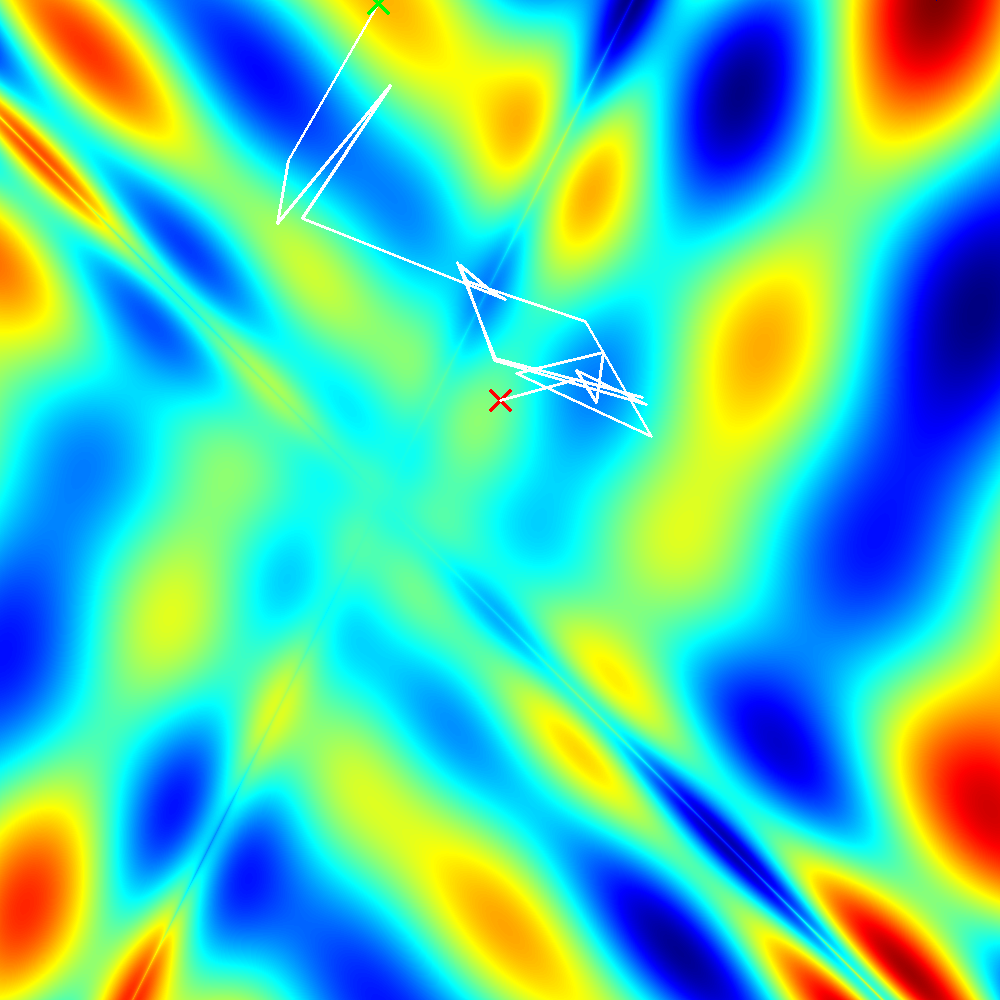
\includegraphics[width=\textwidth]{divergence.png}
    \subcaption{Divergence}
  \end{subfigure}
\vspace{-.7\baselineskip}
\caption{Problems with gradient descent}
\label{p1:problems}
\end{figure}

The function \emph{eggholder} is a a function with many local minima,
and figure \ref{p1:problems}(a) shows how gradient descent reacts to this.

The length of the step is influenced by the so-called \emph{learning rate}.
Essentially this is a factor which is used to multiply the gradient vector.
A large learning rate should help finding a minimum faster - the method
is then making larger steps towards the solution.
Sometimes, however, larger learning rates can influence the convergence negatively:
the method sometimes is oscillating around the final solution before converging.
This can be seen in figure \ref{p1:problems}(b).
And an even higher learning rate might cause divergence of the solution,
where the parameters leave the range of valid values.
An example for this is displayed in figure \ref{p1:problems}(c).

Starting from the simple gradient descent architecture there
are more refined optimizers.
One possibility is adding \emph{momentum} which accelerates
the optimizer into the direction of past movement.
Momentum will find the solution without having to specify
a larger learning rate.
The way momentum influences the search for the solution can
be seen in figure \ref{p1:momentum}.

\begin{figure}[ht]
\begin{subfigure}[c]{0.45\columnwidth}
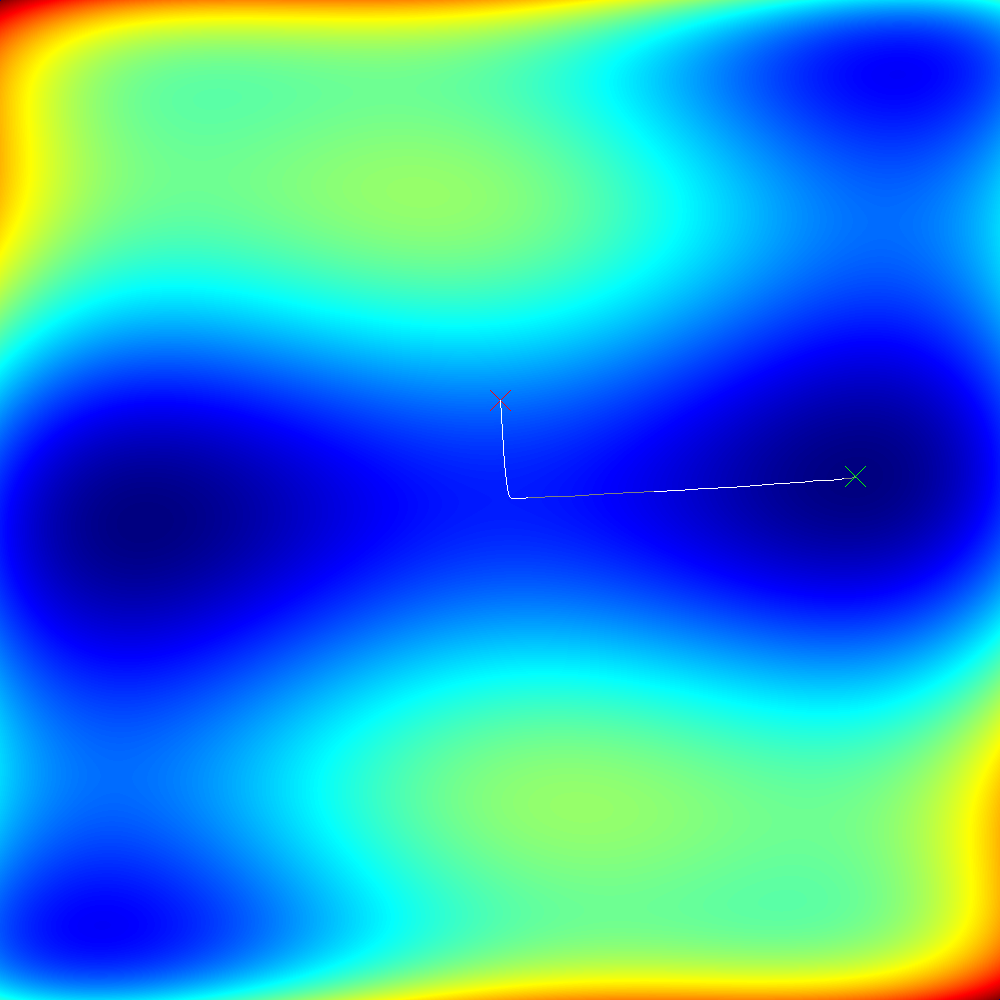
\includegraphics[width=\textwidth]{sgd-camel-nomomentum.png}
\subcaption{Without momentum}
\end{subfigure}
\hspace{2pt}
\begin{subfigure}[c]{0.45\columnwidth}
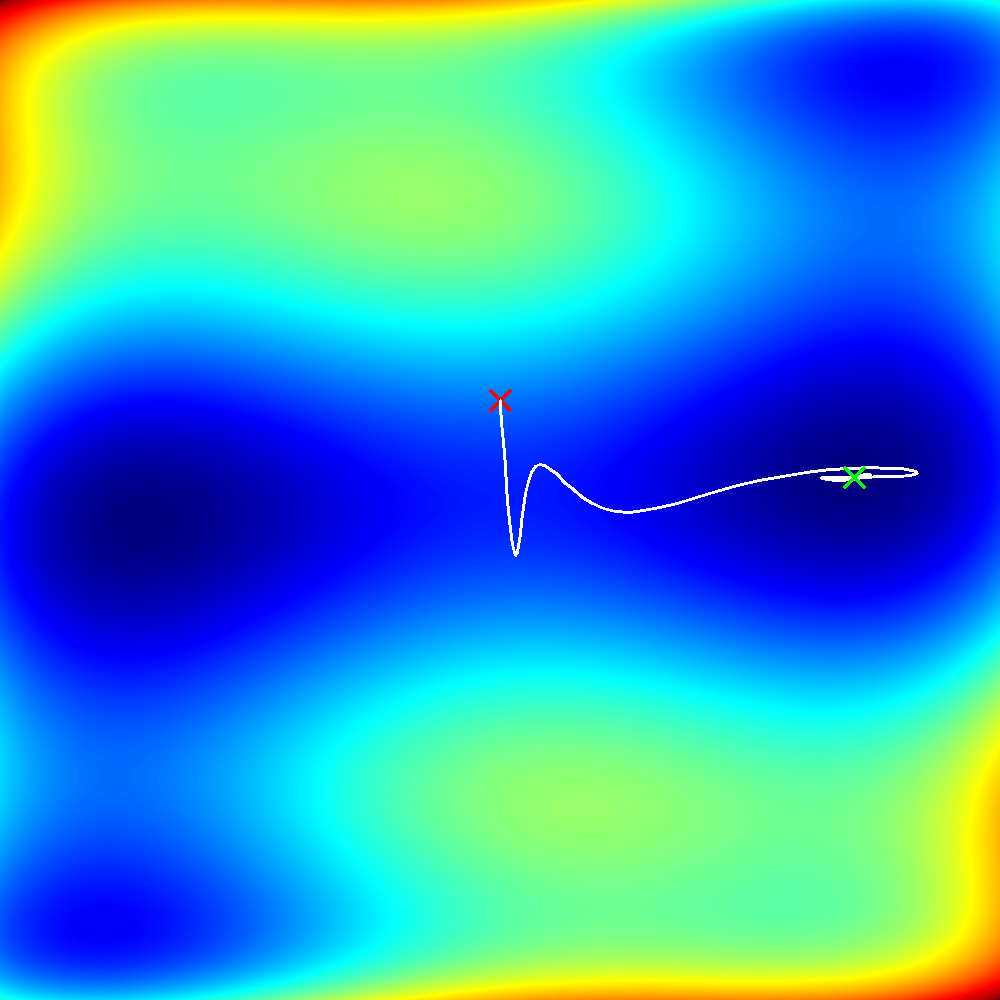
\includegraphics[width=\textwidth]{sgd-camel-momentum.png}
\subcaption{With momentum}
\end{subfigure}
\vspace{-.7\baselineskip}
\caption{Influence of momentum}
\label{p1:momentum}
\end{figure}

One very famous architecture is called Adam - adaptive moment estimation.
It was proposed first in \cite{kingma2014adam}.
It usually converges more directly to the solution than
regular gradient descent, both with and without momentum.

\begin{figure}[ht]
\begin{subfigure}[c]{0.45\columnwidth}
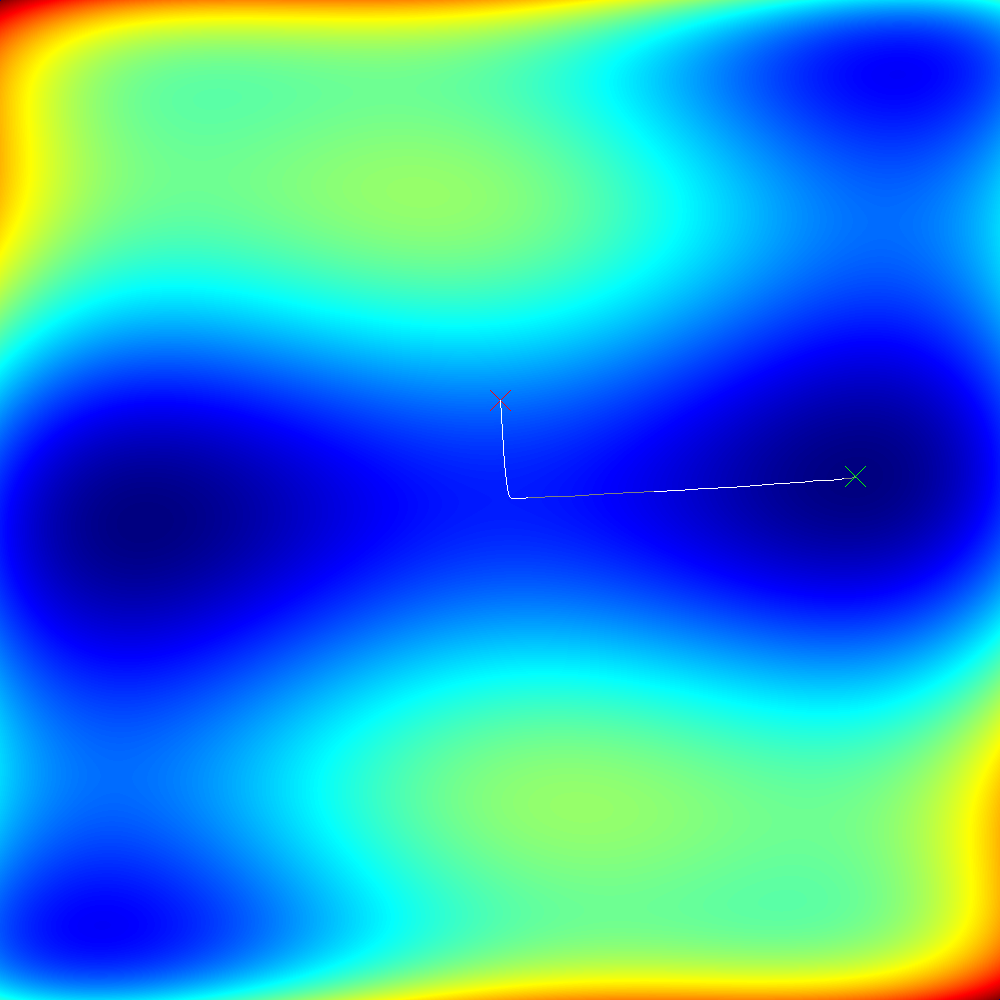
\includegraphics[width=\textwidth]{sgd-camel-nomomentum.png}
\subcaption{Gradient descent}
\end{subfigure}
\hspace{2pt}
\begin{subfigure}[c]{0.45\columnwidth}
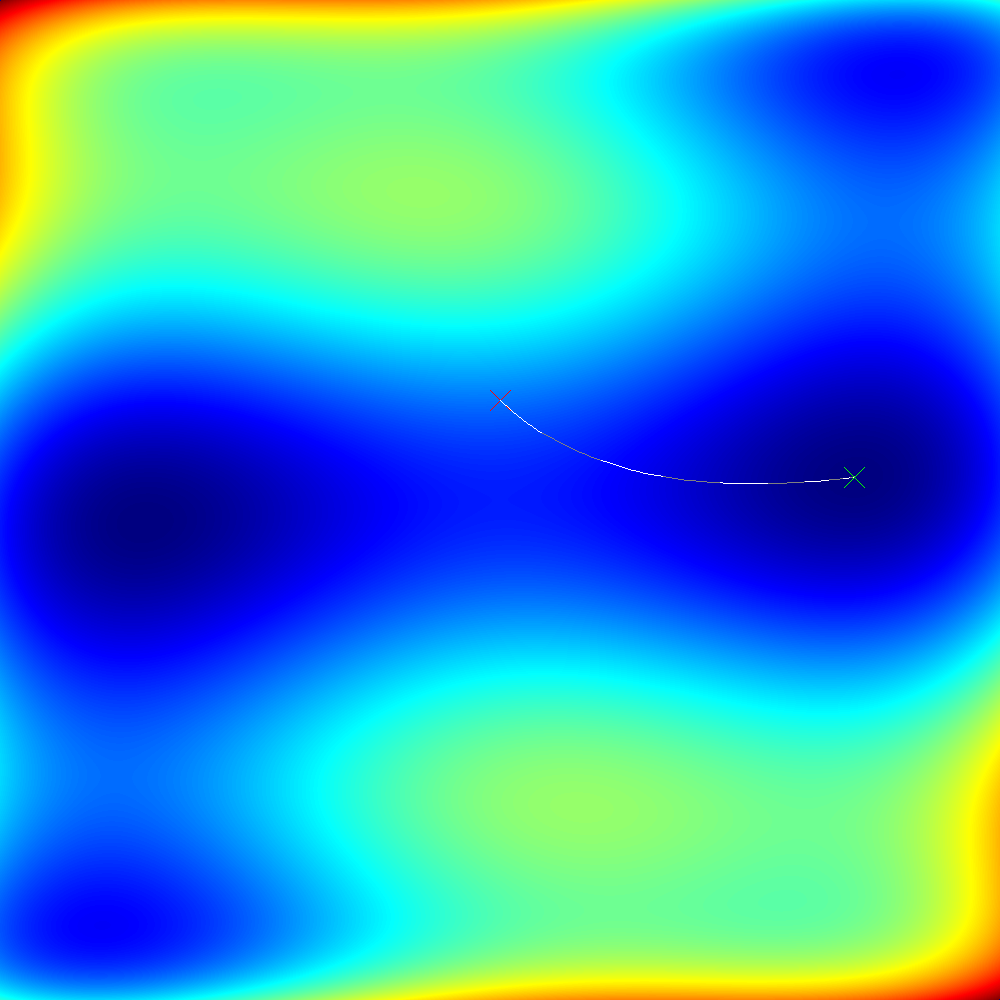
\includegraphics[width=\textwidth]{adam-camel.png}
\subcaption{Adam}
\end{subfigure}
\vspace{-.7\baselineskip}
\caption{Adam vs. gradient descent}
\label{p1:momentum}
\end{figure}

\section{Network Architecture}

For this part of the exercise we were
experimenting with three convolutional neural networks.
The first one, our baseline network, was
based on the suggested network from the slides.

\begin{figure}[ht]
  \begin{subfigure}[t]{0.3\columnwidth}
    \scriptsize
    \begin{tabular}{l}
      Layers \\
      \hline
      Conv2d(64,k=7,p=3,s=2) \\
      ReLU  \\
      MaxPool2d(k=2,s=2) \\
      Conv2d(128,k=3,p=1,s=1) \\
      ReLU \\
      Conv2d(128,k=3,p=1)  \\
      ReLU \\
      MaxPool2d(k=2,s=2) \\
      Conv2d(256,k=3,p=1) \\
      ReLU \\
      Conv2d(256,k=3,p=1) \\
      ReLU \\
      MaxPool2d(k=2,s=2) \\
      AvgPool2d(k=2) \\
      Flatten \\
      Linear(2) \\
      ~\\
      ~\\
      ~\\
      ~\\
    \end{tabular}
    \subcaption{Baseline model}
  \end{subfigure}
  \begin{subfigure}[t]{0.3\columnwidth}
    \scriptsize
    \begin{tabular}{l}
      Layers \\
      \hline
      Conv2d(64,k=7,p=3,s=2) \\
      ReLU  \\
      MaxPool2d(k=2,s=2) \\
      AvgPool2d(k=2) \\
      Flatten \\
      Linear(2) \\
      ~\\
      ~\\
      ~\\
      ~\\
      ~\\
      ~\\
      ~\\
      ~\\
      ~\\
      ~\\
      ~\\
      ~\\
      ~\\
      ~\\
    \end{tabular}
    \subcaption{Simple model}
  \end{subfigure}
  \begin{subfigure}[t]{0.3\columnwidth}
    \scriptsize
    \begin{tabular}{l}
      Layers \\
      \hline
      Conv2d(64,k=7,p=3,s=2) \\
      ReLU  \\
      MaxPool2d(k=2,s=2) \\
      Conv2d(128,k=3,p=1,s=1) \\
      ReLU \\
      Conv2d(128,k=3,p=1)  \\
      ReLU \\
      MaxPool2d(k=2,s=2) \\
      Conv2d(256,k=3,p=1) \\
      ReLU \\
      Conv2d(256,k=3,p=1) \\
      ReLU \\
      MaxPool2d(k=2,s=2) \\
      Conv2d(512,k=3,p=1) \\
      ReLU \\
      Conv2d(512,k=3,p=1) \\
      ReLU \\
      MaxPool2d(k=2,s=2) \\
      Flatten \\
      Linear(2) 
    \end{tabular}
    \subcaption{Complex model}
  \end{subfigure}
  \label{part2:networks}
\vspace{-.7\baselineskip}
  \caption{Network designs}
\end{figure}


As a second network we designed a simplified version, using
just one convolutional layer with max- and average-pooling.
And a third network was based on the slides, with an
additional ``block,'' to see how the network complexity
influences the accuracy and the training success.
When running the experiments the three networks
were behaving as expected (see \ref{part2:network}): the simple network could not
reach the full success due to its oversimplification,
the larger network due to its overcomplexity and the
correspondig lack of training data,
and the baseline network generally achieved the best
results.

\begin{figure}[ht]
\begin{subfigure}[c]{0.3\columnwidth}
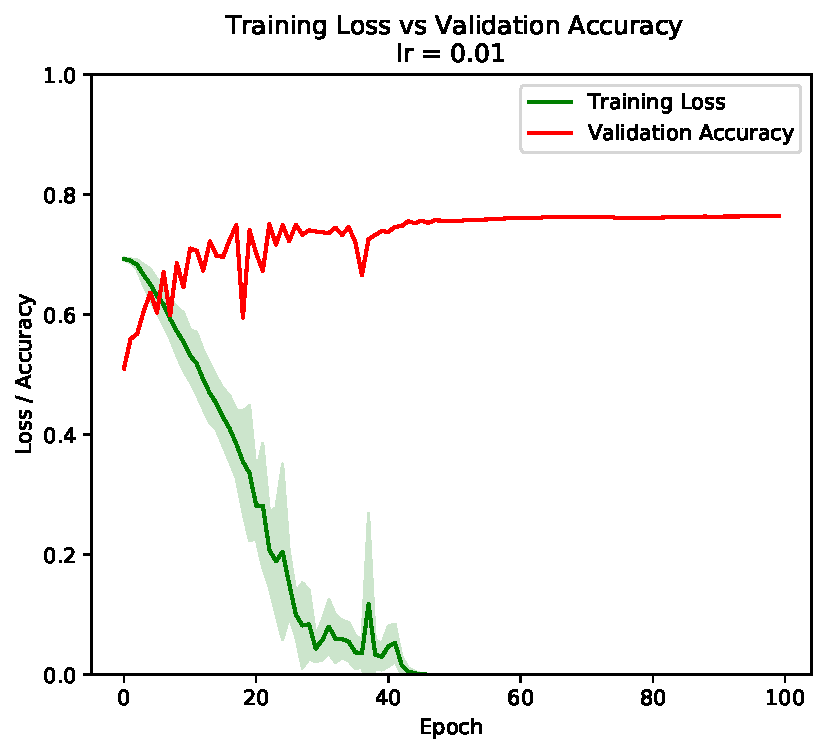
\includegraphics[width=\textwidth]{plot_0_01.pdf}
\subcaption{Baseline (0.765)}
\end{subfigure}
\hspace{1pt}
\begin{subfigure}[c]{0.3\columnwidth}
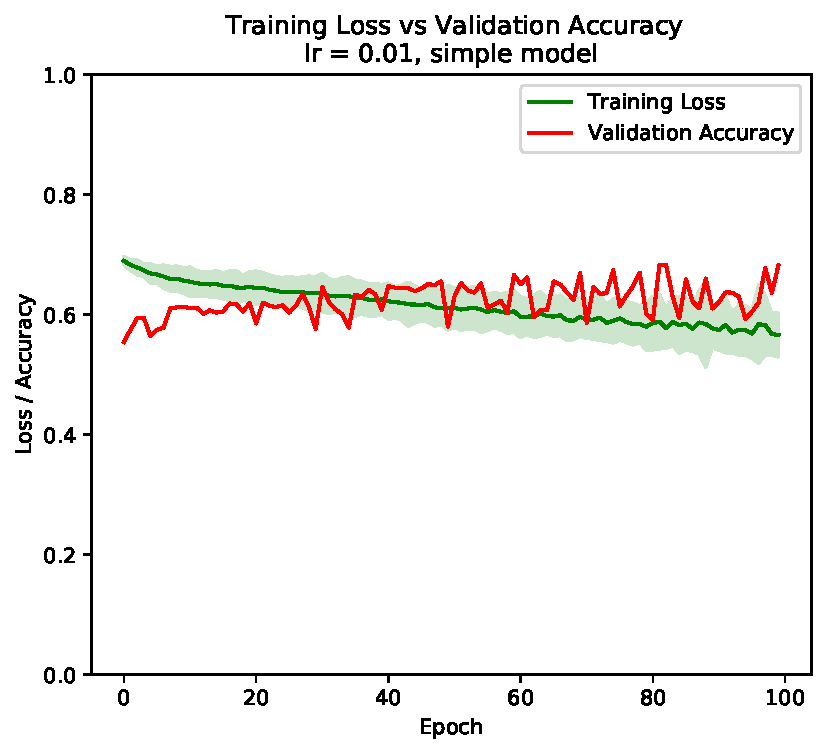
\includegraphics[width=\textwidth]{plot_simple_0_01.pdf}
\subcaption{Simple (0.683)}
\end{subfigure}
\hspace{2pt}
\begin{subfigure}[c]{0.3\columnwidth}
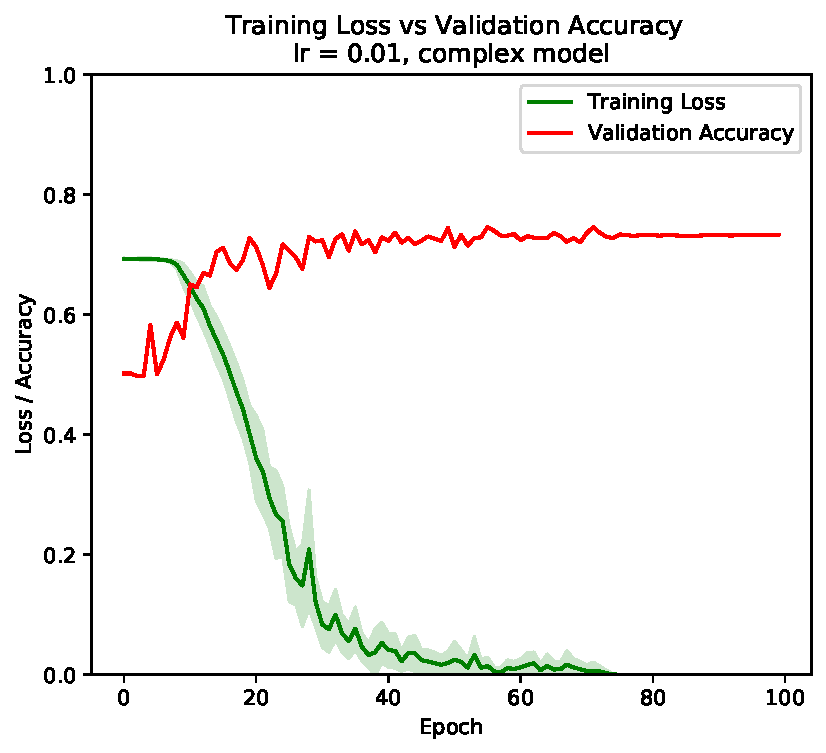
\includegraphics[width=\textwidth]{plot_complex_0_01.pdf}
\subcaption{Complex (0.733)}
\end{subfigure}
\vspace{-.7\baselineskip}
\caption{Comparing networks and final validation accuracy}
\label{part2:network}
\end{figure}
  
We also made experiments with different learning rates,
from a very low learning rate (0.0001) where the
100 epochs of training were not sufficient up to an
extremely high learning rate (0.5) where sometimes the
training failed due to some parameters becoming
``\emph{nan}''-values. This can be seen in
\ref{part2:learning-rate}.
As a general observation we saw that higher learning
rate leads to a higher fluctuation in both training
loss and validation accuracy - we explain this
with the oscillating behavior we experienced in
part 1 of the assignment.

\begin{figure}[ht]
\begin{subfigure}[c]{0.45\columnwidth}
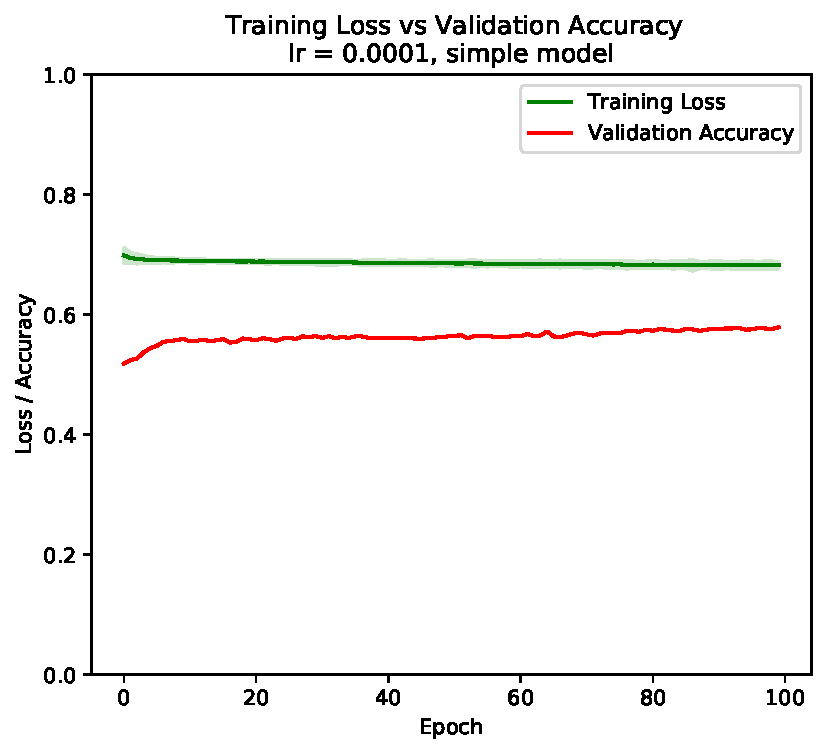
\includegraphics[width=\textwidth]{plot_simple_0_0001.pdf}
\subcaption{Too small}
\end{subfigure}
\hspace{2pt}
\begin{subfigure}[c]{0.45\columnwidth}
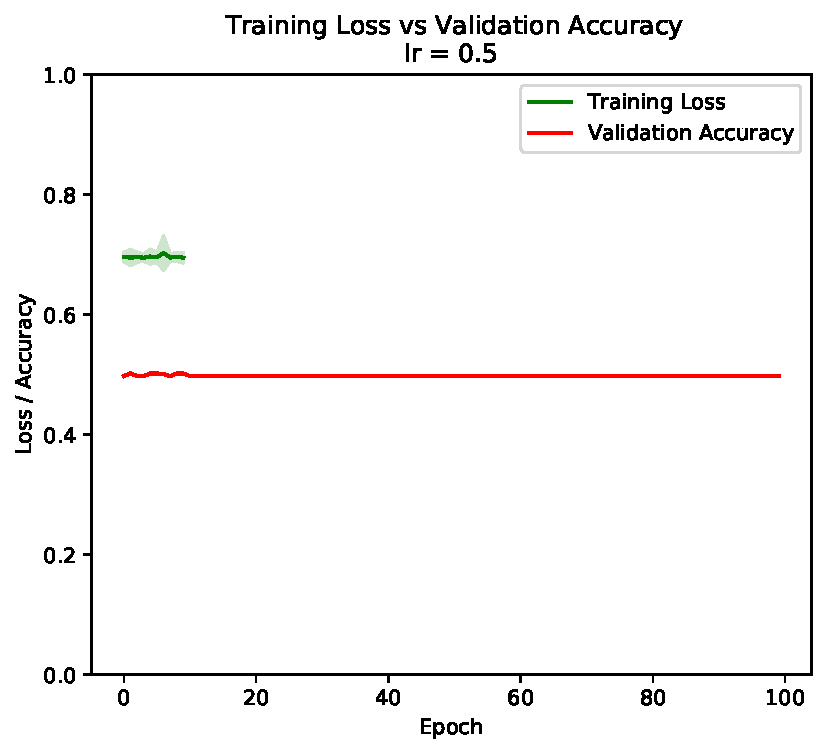
\includegraphics[width=\textwidth]{plot_0_5.pdf}
\subcaption{Too high}
\end{subfigure}
\vspace{-.7\baselineskip}
\caption{Impact of extreme learning rate values}
\label{part2:learning-rate}
\end{figure}

Another type of experiments was related with the
preprocessing, specifically the scaling of the
samples.
The first version was using the suggested scaling 
using a fixed multiplication / addition to bring the
values into the range $[-1,1]$.
The second version, which we generally used for the
other experiments, was using the training
per-channel means and variances to scale the samples
into a mean of 0 and a standard deviation of 1.
The differences were actually not that large,
with different results depending on network and
learning rate.

\begin{figure}[ht]
\begin{subfigure}[c]{0.45\columnwidth}
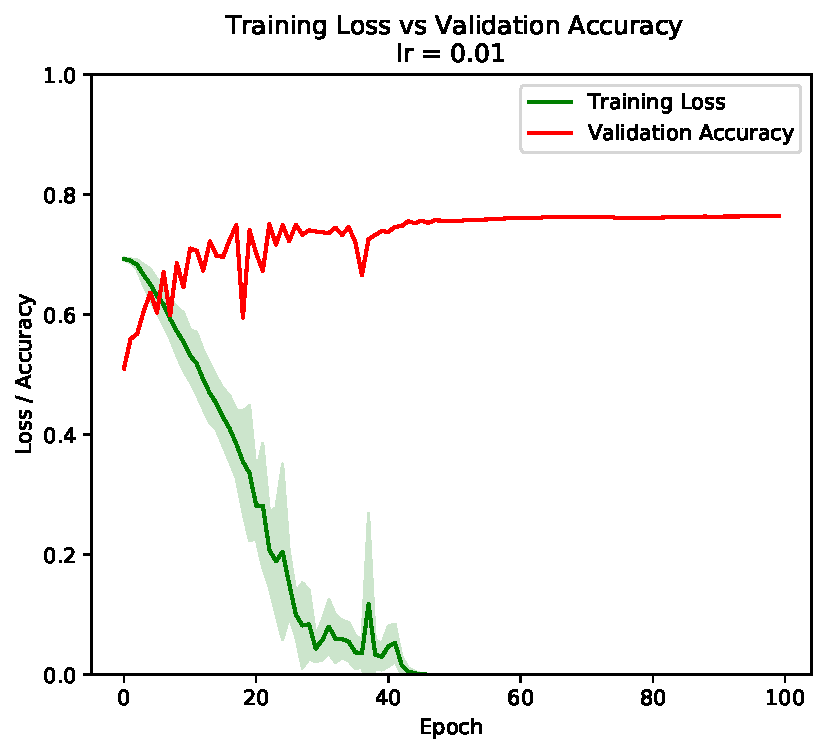
\includegraphics[width=\textwidth]{plot_0_01.pdf}
\subcaption{Regular model}
\end{subfigure}
\hspace{2pt}
\begin{subfigure}[c]{0.45\columnwidth}
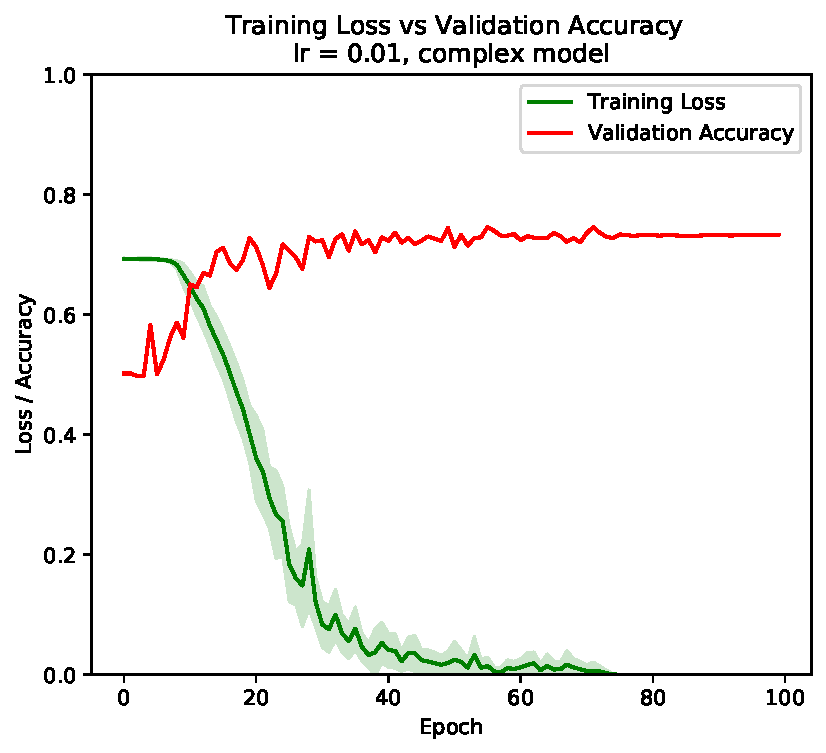
\includegraphics[width=\textwidth]{plot_complex_0_01.pdf}
\subcaption{Complex model}
\end{subfigure}
\vspace{-.7\baselineskip}
\caption{Converging models}
\label{part2:converging}
\end{figure}

\section{Avoiding of Overfitting}


Overall, we reached a final validation accuracy of 0.77.
The baseline and complex networks easily reached a
training loss of 0 after some epochs, showing that
they could not learn anymore from the training data.
The difference between this low training loss and
the final error (1-accuracy) in the validation
is a clear sign of overfitting.

We therefore experimented with methods for avoiding
overfitting, starting with data augmentation,
model regularization and early stopping.

\subsection{Data Augmentation}

For the data augmentation we added random variations of
the training data within the batch generator.
The variations implemented were:
\begin{itemize}
\item Random horizontal flipping
\item Random cropping (padding 5 pixels first)
\item Random rotation (+/- 10 degree)
\item Random zooming (+/- 10\%)
\item Random lightness change (+/- 10\%)
\item Random noise (+/- 0.05)
\end{itemize}

These modifications were fed into the training process
but not into the evaluation using the validation data.

With data augmentation, the complex network was making the
most progress. In one round (learning rate 0.05) it was
reaching a final validation accuracy of 0.77.
For the other models the data augmentation did
not improve the results.
However, as can be seen in \ref{part2:augmentation},
the training process was clearly different,
with the training loss not reaching zero.
Due to the variations in the training samples
the network was able to learn
more and more with each epoch.

\begin{figure}[ht]
\begin{subfigure}[c]{0.45\columnwidth}
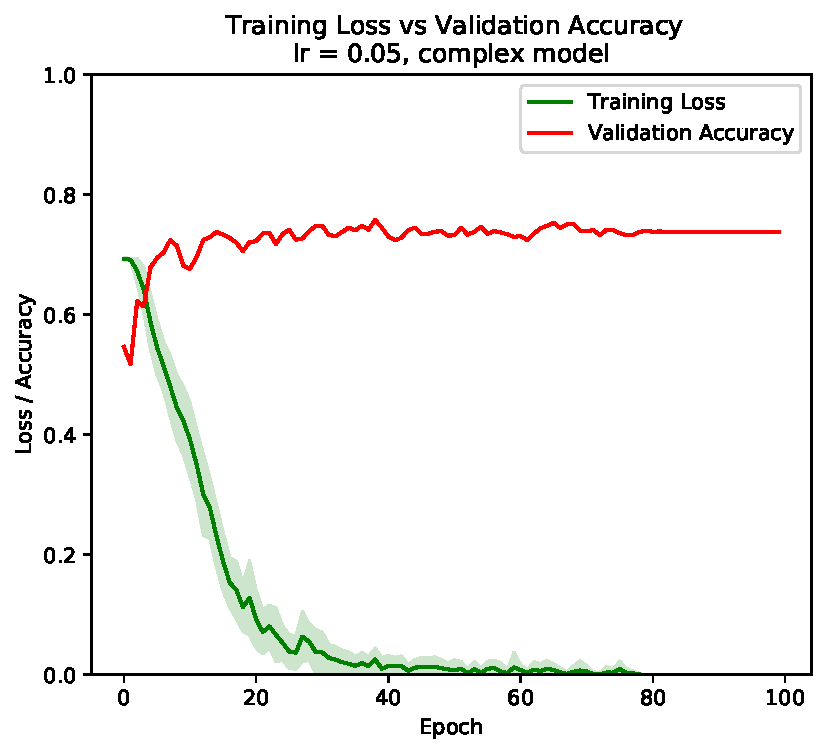
\includegraphics[width=\textwidth]{plot_complex_0_05.pdf}
\subcaption{Without augmentation}
\end{subfigure}
\hspace{2pt}
\begin{subfigure}[c]{0.45\columnwidth}
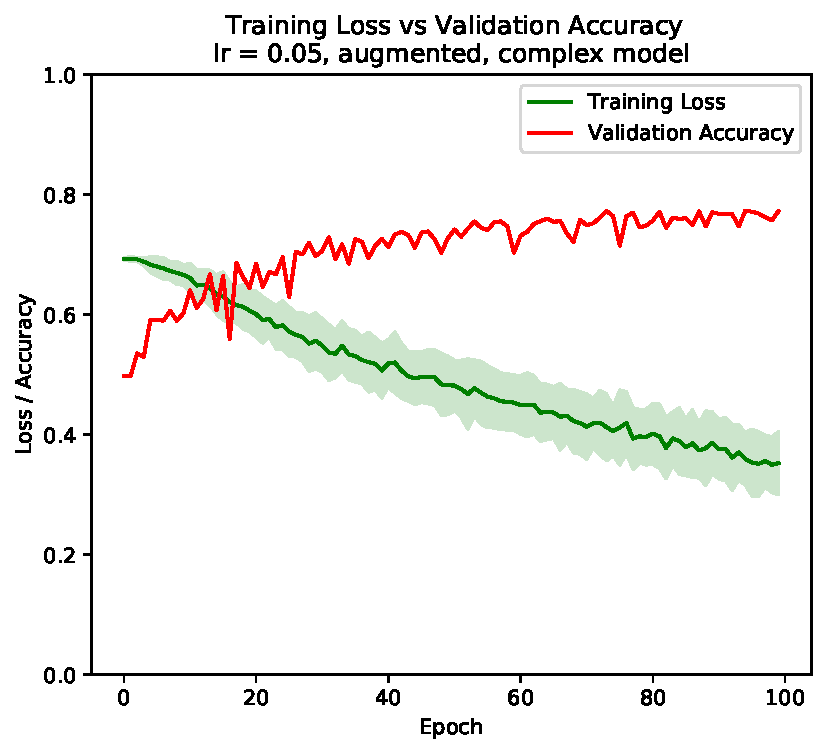
\includegraphics[width=\textwidth]{plot_augmented_complex_0_05.pdf}
\subcaption{With augmentation}
\end{subfigure}
\vspace{-.7\baselineskip}
\caption{Data augmentation}
\label{part2:augmentation}
\end{figure}
  
\subsection{Regularization}

Another approach trying to counter the impact of overfitting
is model regularization.

There are two experiments we conducted here:
using weight decay (or L2 regularization)
and dropout.

\subsubsection{L2-regularization}
In the training the function - which is optimized 
using gradient descent - is amended
with a regularization term, the L2-norm of the parameters.
This should avoid extreme weights, looking at only
a few features of the data, and instead give a more
even model.

We experimented with different values of this L2-penalty,
also called ``weight decay'': 0.1, 0.01 and 0.001.
The baseline network reached up to 0.779 validation
accuracy (learning rate 0.005, weight decay 0.001),
and the complex network up to 0.748 for the final
validation accuracy (learning rate 0.005, weight
decay 0.001).
A higher weight decay was very negative on the final
accuracy, leading to values around 0.5 (as good
as flipping a coin).

\subsubsection{Dropout}
This method consists
of setting randomly some features in the
network to zero.
Following the recommendation in the slides we have
put the dropout layer just before the last layer
of the networks.

We experimented with values of 10\% and 20\%
for the dropout.
The best results were for the baseline network
0.777 (20\% dropout, learning rate 0.002),
for the simple network 0.689 (10\% dropout, learning rate 0.1),
and for the complex network 0.757 (20\% dropout,
learning rate 0.05).

\subsection{Early Stopping}

Another approach to avoid overfitting is \emph{early stopping}.
Normally this is implemented by stopping the training process
once the validation accuracy is not growing for some time.

Following the assignment text we chose a slightly different
approach.
We keep the model with the highest validation accuracy 
and return it after training with 100 epochs.
This way it will in all cases yield an improvement over
the previous approach, which was just taking the model
after the last epoch.

For the baseline network this yields a validation accuracy
of 0.770, for the simple network 0.693, and for the
complex network 0.758.

\section{Best Model}

We made then various experiments with combining the
approaches.
Early stopping was always taken, as it can only have
a positive impact.
However, weight decay and dropout were competing
methods, and so we analysed them in combination,
also with and without data augmentation.

\section{Transfer Learning}

Finally we made some experiment using transfer
learning.
The idea here is to use weights established from training
of larger data sets and to amend these weights with
a set of final layers which are trained for the purpose.

We chose ResNet18 (\cite{resnet2015}) as our learned
model.
This yielded way superior results to our networks.
The final validation accuracy reached 0.842 (learning
rate 0.01), and when combined with early stopping the best
model had a validation accuracy of 0.865.

Clearly transfer learning is the best approach for
situations with limited training data.

\bibliographystyle{ACM-Reference-Format}
\bibliography{report}
\end{document}
